%%%%%%%%%%%%%%%%%%%%%%%%%%%%%%%%%%%%%%%%%
% University Assignment Title Page 
% LaTeX Template
% Version 2.0 (21/04/18)
% Modified by
% Erdem TUNA &
% Halil TEMURTAŞ
%
% This template has been downloaded from:
% http://www.LaTeXTemplates.com
%
% Original author:

% Instructions for using this template:
% This title page is capable of being compiled as is. This is not useful for 
% including it in another document. To do this, you have two options: 
%
% 1) Copy/paste everything between \begin{document} and \end{document} 
% starting at \begin{titlepage} and paste this into another LaTeX file where you 
% want your title page.
% OR
% 2) Remove everything outside the \begin{titlepage} and \end{titlepage} and 
% move this file to the same directory as the LaTeX file you wish to add it to. 
% Then add \input{./title_page_1.tex} to your LaTeX file where you want your
% title page.
%
%%%%%%%%%%%%%%%%%%%%%%%%%%%%%%%%%%%%%%%%%
%\title{Title page with logo}
%----------------------------------------------------------------------------------------
%	PACKAGES AND OTHER DOCUMENT CONFIGURATIONS
%----------------------------------------------------------------------------------------

\documentclass[a4paper,12pt]{article}
\usepackage[a4paper, total={6.5in, 8in}]{geometry}
%\documentclass[12pt]{article}
\usepackage[english]{babel}
\usepackage[utf8x]{inputenc}
\usepackage{amsmath}
\usepackage{graphicx}
\usepackage[colorinlistoftodos]{todonotes}
\usepackage{gensymb} % this could be problem
\usepackage{float}
\usepackage{fancyref}
\usepackage{subcaption}
\usepackage[toc,page]{appendix} %appendix package
\usepackage{xcolor}
\usepackage{listings}
\usepackage{xspace}


\usepackage{amssymb}
\usepackage{nicefrac}
\usepackage{gensymb}
\usepackage{xspace}
\usepackage{fancyhdr}

%\usepackage{showframe}



\newcommand\nd{\textsuperscript{nd}\xspace}
\newcommand\rd{\textsuperscript{rd}\xspace}
\newcommand\nth{\textsuperscript{th}\xspace} %\th is taken already


\definecolor{mGreen}{rgb}{0,0.6,0} % for python
\definecolor{mGray}{rgb}{0.5,0.5,0.5}
\definecolor{mPurple}{rgb}{0.58,0,0.82}
\definecolor{mygreen}{RGB}{28,172,0} % color values Red, Green, Blue for matlab
\definecolor{mylilas}{RGB}{170,55,241}





\lstdefinestyle{CStyle}{
    commentstyle=\color{mGreen},
    keywordstyle=\color{magenta},
    numberstyle=\tiny\color{mGray},
    stringstyle=\color{mPurple},
    basicstyle=\footnotesize,
    breakatwhitespace=false,         
    breaklines=true,
    frame=single,
    rulecolor=\color{black!40},                 
    captionpos=b,                    
    keepspaces=true,                 
    numbers=left,                    
    numbersep=5pt,                  
    showspaces=false,                
    showstringspaces=false,
    showtabs=false,                  
    tabsize=2,
    language=C
}


\lstset{language=Matlab,%
    %basicstyle=\color{red},
    breaklines=true,%
    frame=single,
    rulecolor=\color{black!40},
    morekeywords={matlab2tikz},
    keywordstyle=\color{blue},%
    morekeywords=[2]{1}, keywordstyle=[2]{\color{black}},
    identifierstyle=\color{black},%
    stringstyle=\color{mylilas},
    commentstyle=\color{mygreen},%
    showstringspaces=false,%without this there will be a symbol in the places where there is a space
    numbers=left,%
    numberstyle={\tiny \color{black}},% size of the numbers
    numbersep=9pt, % this defines how far the numbers are from the text
    emph=[1]{for,end,break},emphstyle=[1]\color{red}, %some words to emphasise
    %emph=[2]{word1,word2}, emphstyle=[2]{style},    
}



\makeatletter
\renewcommand\paragraph{\@startsection{paragraph}{4}{\z@}%
            {-2.5ex\@plus -1ex \@minus -.25ex}%
            {1.25ex \@plus .25ex}%
            {\normalfont\normalsize\bfseries}}
\makeatother
\setcounter{secnumdepth}{5} % how many sectioning levels to assign numbers to
\setcounter{tocdepth}{5}    % how many sectioning levels to show in ToC



% For Blank Page -------------
\newcommand{\blankpage}{
	\- \\[8.5cm]	
	{ \centering This Page Intentionally Left Blank \par }
	\- \\[8.5cm]
}
% ---------------------------


\pagestyle{fancy}
\fancyhf{}
\rhead{\large 10.10.2018 }%\\\ Thursday Afternoon}
\lhead{\large Halil Temurtaş \\ \large 2094522 }
\rfoot{Page \thepage}




\begin{document}


\begin{minipage}{1.0\textwidth}
\center
\- \\[0.5cm]
\textbf{\large EE402 Discrete Time Control Systems \\[0.2cm] Mini-Project 1} \\
\end{minipage}


\begin{enumerate}
	\item For each of the following systems with input u and output y, t $\geq$ 0, determine whether the system is memoryless, linear, time-invariant, causal, finite-dimensional ? 

		\begin{enumerate}
			\item 	$ y(t) = (sin(t))^3	$
			\item 	$ y(t) = \int_{0}^{t} \tau u(\tau) d\tau $ 	
			\item 	$ y(t) = 2u(t)+10$
			\item 	$ y(t) = cos(t)u(t)	$
			\item 	$ y(t) = u(t-T)	$
			\item 	$ y(t) = u[k-n]	$
			\item \-	
				\begin{figure}[H]
					\center
					\setlength{\unitlength}{\textwidth} 
					%\includegraphics[width=0.9\unitlength]{organizasyon2}
					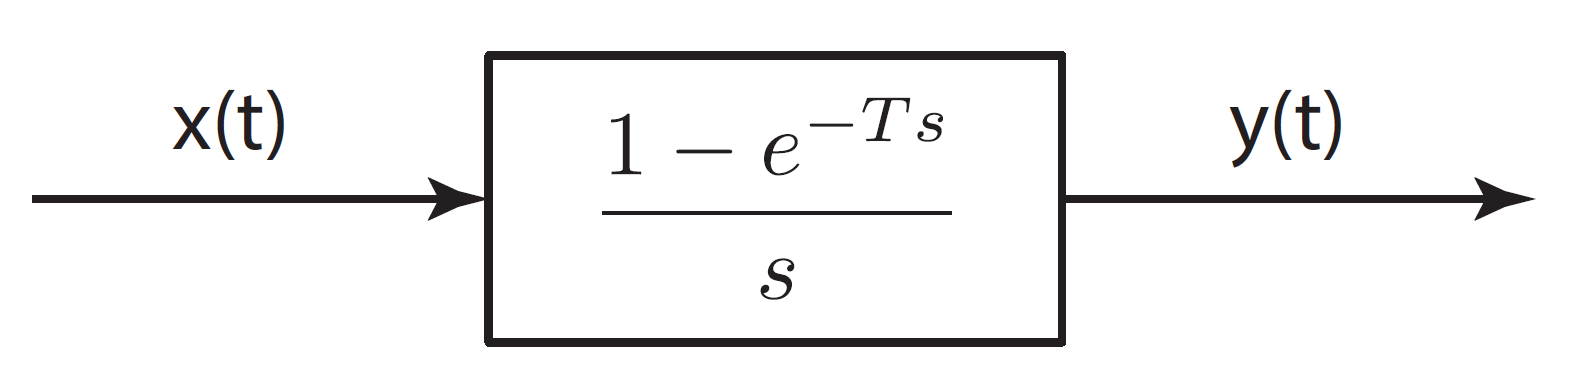
\includegraphics[width=0.6\unitlength]{1g}
					%\caption{\label{fig:orgc}The Organizational Chart of ASELSAN }
				\end{figure}
		\end{enumerate}
	
	
	\item Review of the basic properties of the convolution operation, denoted by *, as well as those of the Laplace transform, denoted by $\mathcal{L}$. Consider   $ f : \mathbb{R} \rightarrow \mathbb{R}$, and  $ g : \mathbb{R} \rightarrow \mathbb{R}$, and  $ h : \mathbb{R} \rightarrow \mathbb{R}$.
		
		\begin{enumerate}
			\item * is associative, that is, $(f * g) * h = f * (g * h)$
			\item $f(t - \tau ) = f(t) * \delta (t - \tau ),\tau \geq 0$, sifting property of the dirac delta function $ \delta (t)$
			\item $ \mathcal{L}(f * g) = \mathcal{L}(f)\mathcal{L}(g) $
			\item $ \mathcal{L}(f + g) = \mathcal{L}(f) + \mathcal{L}(g) $
		\end{enumerate}
	
	
	
		 
	\item Finding $ Y (s)=U(s) $ for the following system
	
	$$ y(t) = \int_{t_T}^{t} h(t-\tau) u(\tau) d\tau $$
	
	\[   
		h(t) = 
     		\begin{cases}
     			t ~~ if ~~ t > 10 \\
     			0 ~~ if ~~ t \leq 0\\
     		\end{cases}
	\]

	\item Analysis of the the control system that is illustrated with the block diagram topology given below. Let's assume that $M(s) = \frac{1}{s-a} , a > 0 $  and $ C(s) = \frac{K}{s+1} $ .
	
	Finding the range of K such that the closed-loop system is stable.
		
	\begin{figure}[H]
		\center
		\setlength{\unitlength}{\textwidth} 
		%\includegraphics[width=0.9\unitlength]{organizasyon2}
		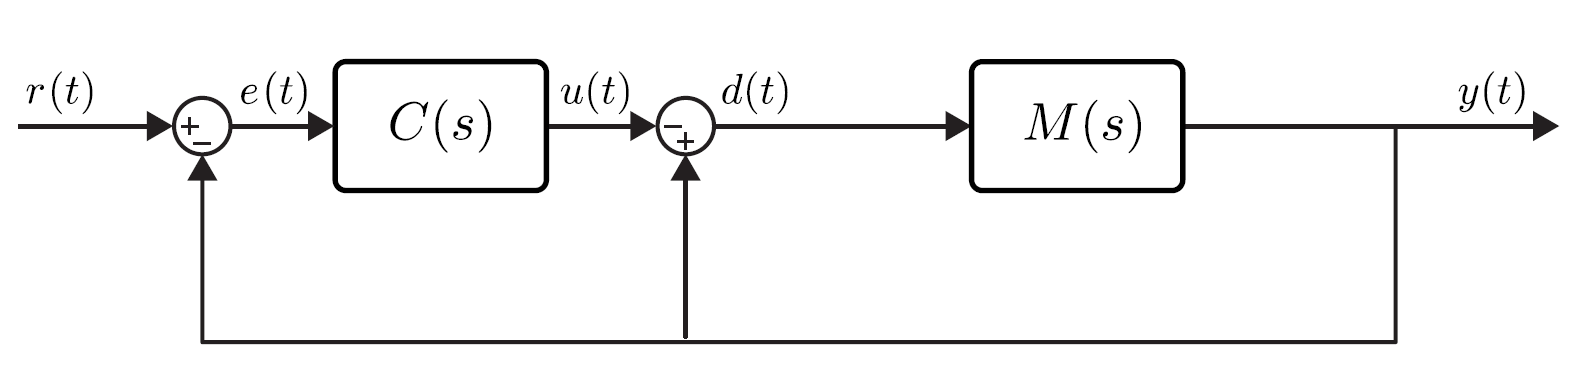
\includegraphics[width=0.6\unitlength]{4}
		%\caption{\label{fig:orgc}The Organizational Chart of ASELSAN }
	\end{figure}
	
	
	\item Inverted pendulum of length L, with mass m, that is actuated by an agonist/antagonist linear actuator pair that attach a distance l from the joint / pivot point. One can show
	
	\begin{minipage}{0.45\textwidth}
		\begin{flushleft} \large
		\[   
		h(t) = 
     		\begin{cases}
     			t ~~ if ~~ t > 10 \\
     			0 ~~ if ~~ t \leq 0\\
     		\end{cases}
	\]
		\end{flushleft}
	\end{minipage}
	\begin{minipage}{0.5\textwidth}
		\begin{flushright} \large
		\begin{figure}[H]
			\center
			\setlength{\unitlength}{\textwidth} 
			%\includegraphics[width=0.9\unitlength]{organizasyon2}
			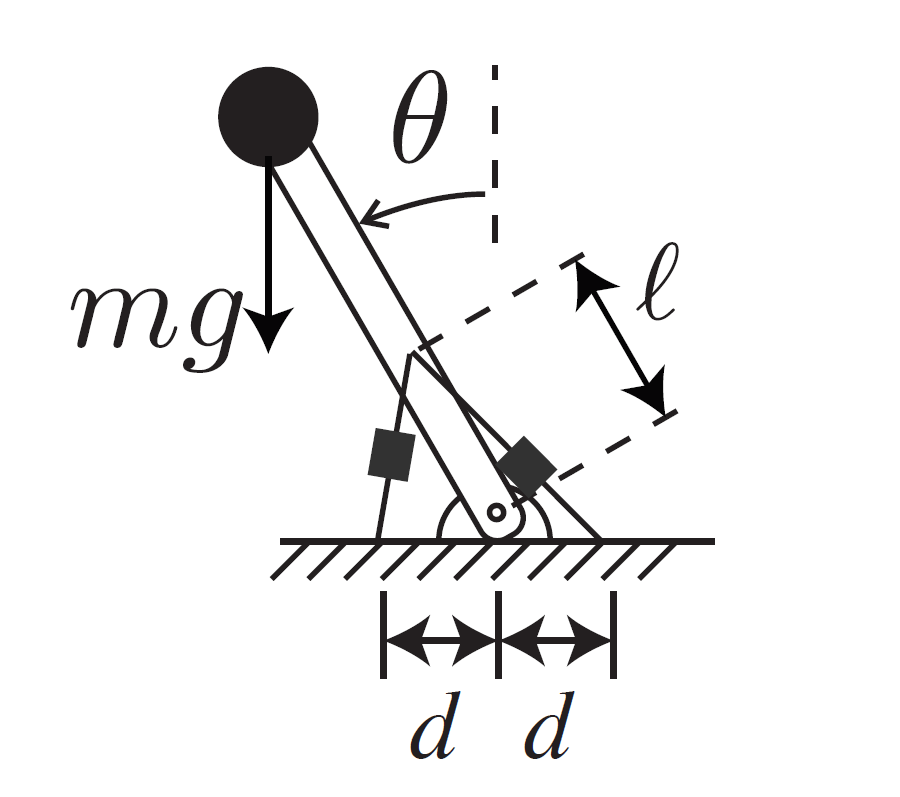
\includegraphics[width=0.6\unitlength]{5}
			%\caption{\label{fig:orgc}The Organizational Chart of ASELSAN }
		\end{figure}
		\end{flushright}
	\end{minipage}



	
	
	

\end{enumerate}

	 	
	

\begin{minipage}{1.0\textwidth}
\center
\- \\[0.5cm]
\textbf{\Large Appendix } 
\end{minipage} 

\- \\[0.5cm]


\lstinputlisting{MP1.m}

%\lstinputlisting[firstline=12, lastline=15]{HW3.m}

%\lstinputlisting[language=Matlab]{HW3.m}


%\lstinputlisting[language=Python, firstline=37, lastline=45]{source_filename.py}

%\begin{lstlisting}[language=Matlab]



%\end{lstlisting}


%\[ \begin{array}{r|rrrrrr}
%s^3 & 3   & 10 & 0 & \cdots & \cdots  \\
%s^2 & 20  & 400 & 0 & \cdots \\
%\hline
%s^1 & -50 & 0 &  \cdots \\
%s^0 & 400 &  \cdots \\
%\end{array} \]



\tikzset{
desicion/.style={
    diamond,
    draw,
    text width=4em,
    text badly centered,
    inner sep=0pt
},
block/.style={
    rectangle,
    draw,
    text width=10em,
    text centered,
    rounded corners
},
cloud/.style={
    draw,
    ellipse,
    minimum height=2em
},
descr/.style={
    fill=white,
    inner sep=2.5pt
},
connector/.style={
    -latex,
    font=\scriptsize
},
rectangle connector/.style={
    connector,
    to path={(\tikztostart) -- ++(#1,0pt) \tikztonodes |- (\tikztotarget) },
    pos=0.5
},
rectangle connector/.default=-2cm,
straight connector/.style={
    connector,
    to path=--(\tikztotarget) \tikztonodes
}
}

\tikzset{
desicion/.style={
    diamond,
    draw,
    text width=4em,
    text badly centered,
    inner sep=0pt
},
block/.style={
    rectangle,
    draw,
    text width=10em,
    text centered,
    rounded corners
},
cloud/.style={
    draw,
    ellipse,
    minimum height=2em
},
descr/.style={
    fill=white,
    inner sep=2.5pt
},
connector/.style={
    -latex,
    font=\scriptsize
},
rectangle connector/.style={
    connector,
    to path={(\tikztostart) -- ++(#1,0pt) \tikztonodes |- (\tikztotarget) },
    pos=0.5
},
rectangle connector/.default=-2cm,
straight connector/.style={
    connector,
    to path=--(\tikztotarget) \tikztonodes
}
}

\vfill


\end{document}
